\section{Exemple de graphique pour la section~\ref{pente-coeff_sec}}
	\begin{figure}[h]
		\centering 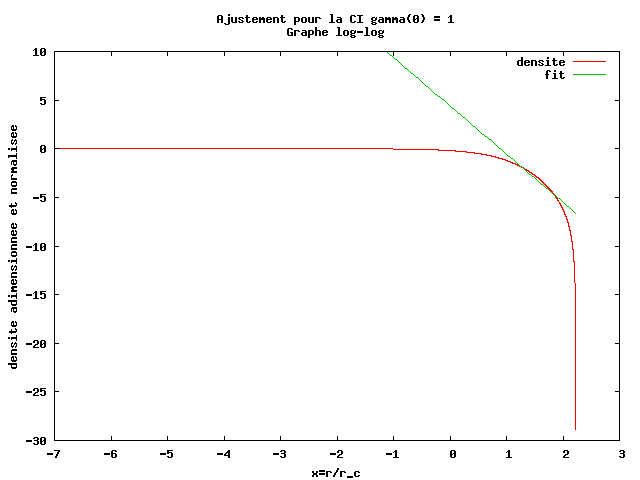
\includegraphics[scale=0.40]{graphe/ci-pente_1.png}
		\caption{Évolution des pentes pour différentes conditions initiales}
		\label{ci-pente_1}
	\end{figure}

	\begin{figure}[h]
		\centering 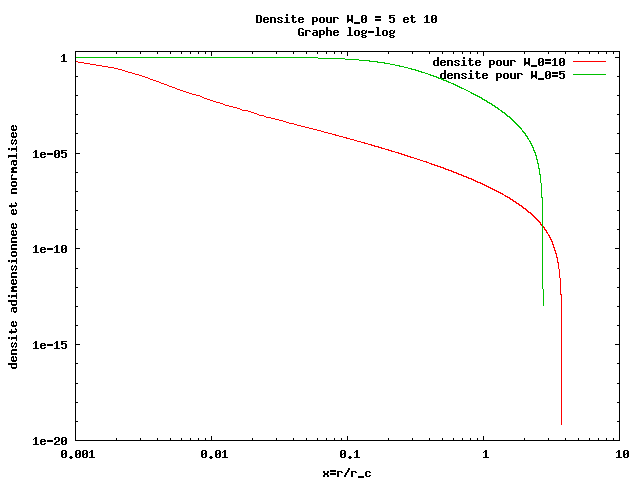
\includegraphics[scale=0.40]{graphe/w_0-5_10.png}
		\caption{Densités pour $W_0 = 5$ et $W_0 = 10$}
		\label{w_0-5_10}
	\end{figure}
	\FloatBarrier

%\section{Tables de données de la section~\ref{pente-coeff_sec}}
%	\markboth{\MakeUppercase{\sectionname}\ \thesection.\ Tables de Données}{}
%	\begin{table}[h]
%		\begin{minipage}[b]{0.30\linewidth}
			%\centering \lstinputlisting{../Res/coeff2.res}
			%\begin{center}
			%	\lstinputlisting{../Res/coeff2.res}
			%\end{center}
			%\caption{Données des graphiques~\ref{coeff_evo} et~\ref{coeur_evo}}
%			\input{table/coeff2.tex}
%		\end{minipage}\hfill
%		\begin{minipage}[b]{0.40\linewidth}
			%\centering \lstinputlisting{../Res/coeff3.res}
			%\begin{center}
			%	\lstinputlisting{../Res/coeff3.res}
			%\end{center}
			%\caption{Données des graphiques~\ref{coeff_evo} et~\ref{coeur_evo2}}
%			\input{table/coeff3.tex}
%		\end{minipage}
%	\end{table}
%	\FloatBarrier
%\newpage
\section{Densité de NGC 5024 et NGC 5139\label{Graphe-bofbof}}
	\begin{figure}[h]
		\centering \includegraphics[scale=1.00]{graphe/NGC5024.pdf}
		\caption{Densité de NGC 5024}
	\end{figure}

	\begin{figure}[h]
		\centering \includegraphics[scale=1.00]{graphe/NGC5139.pdf}
		\caption{Densité de NGC 5139}
	\end{figure}
	\FloatBarrier

%\section{Tables pour la section~\ref{amas}}
%	\markboth{\MakeUppercase{\sectionname}\ \thesection.\ Tables de Données}{}
%	\begin{landscape}
%		\setlongtables
%		\input{../Amas/table-pente.tex}
%	\end{landscape}
%	\input{table/pente-Tc.tex}
%	\input{table/pente-dim.tex}

%	\begin{landscape}
%		\setlongtables
%		\input{../Catalogue_Harris/Cata.tex}
%		\caption{Données utilisées du catalogue de Harris\label{Harris-cat}}
%	\end{landscape}

\section{Résultat de simulation}
\subsection{Profils de densité}
\begin{figure}[h!]
	\centering \includegraphics[scale=0.5]{graphe/Comp_dens_gene-theo_0-019.pdf}
	\caption{Comparaison entre la densité numérique et la densité après évolution : $\epsilon = 0.0194028$\label{soft::0.019}}
\end{figure}


\begin{figure}[h!]
	\centering \includegraphics[scale=0.5]{graphe/Comp_dens_gene-theo_0-15.pdf}
	\caption{Comparaison entre la densité numérique et la densité après évolution : $\epsilon = 0.15$\label{soft::0.15}}
\end{figure}


\begin{figure}[h!]
	\centering \includegraphics[scale=0.5]{graphe/Comp_dens_gene-theo_0-2.pdf}
	\caption{Comparaison entre la densité numérique et la densité après évolution : $\epsilon = 0.2$\label{soft::0.2}}
\end{figure}


\begin{figure}[h!]
	\centering \includegraphics[scale=0.5]{graphe/Comp_dens_gene-theo_0-3.pdf}
	\caption{Comparaison entre la densité numérique et la densité après évolution : $\epsilon = 0.3$\label{soft::0.3}}
\end{figure}

	\FloatBarrier

\subsection{Évolution des axes d'inertie}
\begin{figure}[h!]
	\centering \includegraphics[scale=0.5]{graphe/Axial_ratio_0-019.pdf}
	\caption{Évolution des rapports des axes d'inertie : $\epsilon = 0.0194028$\label{soft::0.019-Ax}}
\end{figure}


\begin{figure}[h!]
	\centering \includegraphics[scale=0.5]{graphe/Axial_ratio_0-15.pdf}
	\caption{Évolution des rapports des axes d'inertie : $\epsilon = 0.15$\label{soft::0.15-Ax}}
\end{figure}


\begin{figure}[h!]
	\centering \includegraphics[scale=0.5]{graphe/Axial_ratio_0-2.pdf}
	\caption{Évolution des rapports des axes d'inertie : $\epsilon = 0.2$\label{soft::0.2-Ax}}
\end{figure}


\begin{figure}[h!]
	\centering \includegraphics[scale=0.5]{graphe/Axial_ratio_0-3.pdf}
	\caption{Évolution des rapports des axes d'inertie : $\epsilon = 0.3$\label{soft::0.3-Ax}}
\end{figure}

